\section{Results}
\label{sec:results}

\subsection{Size sweep: mAP saturates, the operating point does not}
\label{sec:size}

Table~\ref{tab:size} reports both depths. The mAP columns are almost flat:
$0.977 \pm 0.003$ for \texttt{yolov8s} over three seeds and $0.979$ for
\texttt{yolov8n} at one seed. On validation the gap is larger
($0.954$ vs.\ $0.932$), which means we cannot claim the smaller model is better
on this evidence: the difference is inside the seed spread of the larger model,
and a single-seed estimate on $189$ test images cannot resolve it. The defensible
reading is that mAP$_{50}$ cannot distinguish the two detectors.

\begin{table}[t]
\centering
\small
\caption{Size sweep on the frozen test split. \texttt{s} is mean $\pm$ std over
seeds $0/1/2$; \texttt{n} is seed $0$ only and therefore carries no interval.
``OP'' is the validation-chosen recall-first operating point
($R\ge0.97$ on validation), applied unchanged to test. Latency is PC GPU FP32,
$640\times640$, median of $50$ runs.}
\label{tab:size}
\scriptsize
\setlength{\tabcolsep}{3pt}
\begin{tabular}{lrrrrrrrrr}
\toprule
model & params & GFLOPs & MB & ms & val mAP$_{50}$ & test mAP$_{50}$ & $R$ & $P$ & FP/img \\
\midrule
yolov8s & 11.1\,M & 28.6 & 21.5 & 6.5 & $0.9544\pm0.0027$ & $0.9768\pm0.0034$ & $0.9763\pm0.0040$ & $0.5157\pm0.2180$ & $1.510\pm1.009$ \\
yolov8n & 3.0\,M & 8.2 & 6.0 & 6.9 & 0.9322 & 0.9787 & 0.9842 & 0.1686 & 6.497 \\
\bottomrule
\end{tabular}
\end{table}

The operating-point columns are not flat at all. At the recall-first point the
smaller detector emits \fpn\ false positives per image against \fps\ for the
larger one---a $4.3\times$ difference, and notice the direction: the model with
fewer parameters is \emph{worse} at deployment while being equal or better on
mAP. Its precision at that point is $0.169$ against $0.516$. The mAP$_{50}$ of
$0.979$ is earned by ranking, not by calibration, and at a fixed high-recall
threshold the ranking advantage evaporates.

This is the paper's central empirical claim, and it is a claim about evaluation.
A benchmark that reports only mAP$_{50}$ would rank \texttt{yolov8n} first and
recommend it for a $8.2$\,GFLOP budget; a deployment engineer would get a
detector emitting four times as many alarms per frame. We note one more
inconvenient detail: measured latency does not favour the smaller model
($6.9$ vs.\ $6.5$\,ms), because at this size the fixed per-image overhead
dominates. The GFLOP and parameter savings are real, the wall-clock saving on
this hardware is not. Reporting FLOPs as a proxy for latency is another summary
statistic that fails to transfer.

\begin{table}[t]
\centering
\small
\caption{Per-seed operating points for \texttt{yolov8s}. The threshold chosen on
validation varies by an order of magnitude across seeds ($0.01$ to $0.21$) and
so does the resulting precision. Test mAP barely moves.}
\label{tab:seed}
\begin{tabular}{lcccccc}
\toprule
seed & val conf & test mAP$_{50}$ & box $P$ & box $R$ & FP/img & image $R$ [95\% CI] \\
\midrule
0 & 0.020 & 0.9741 & 0.427 & 0.976 & 1.751 & 1.000 [0.980, 1.000] \\
1 & 0.010 & 0.9807 & 0.356 & 0.980 & 2.376 & 0.995 [0.970, 0.999] \\
2 & 0.210 & 0.9756 & 0.764 & 0.972 & 0.402 & 0.984 [0.953, 0.994] \\
\bottomrule
\end{tabular}
\end{table}

Table~\ref{tab:seed} exposes the mechanism. The three seeds reach nearly identical
test mAP ($0.974$--$0.981$) and nearly identical recall ($0.972$--$0.980$), but
the validation procedure selects thresholds of $0.02$, $0.01$, and $0.21$,
producing precisions of $0.427$, $0.356$, and $0.764$. Seed 2 is eight to ten
times more conservative at the same mAP. Any claim about ``the model's precision''
that pools these seeds is a claim about the threshold-selection procedure, not
about the detector. We therefore report per-seed values wherever precision or
FP/image is the quantity of interest, and treat the three-seed mean as a summary
of protocol variance rather than of model quality.

\subsection{Where the variance lives: source structure}
\label{sec:persource}

The source-cluster bootstrap makes the same point from a different direction. For
seed 0, resampling the three test sources gives $P \in [0.195, 0.874]$,
$R \in [0.948, 1.000]$, and $\mathrm{FP/img} \in [0.139, 30.1]$. With three
clusters these intervals are honest but almost uninformative; the
leave-one-source-out analysis is more legible. Removing \texttt{Jan\_lwir}---the
ten images that generate most of the false alarms---raises seed-0 precision from
$0.427$ to $0.853$ and drops FP/image from $1.75$ to $0.17$. Removing
\texttt{ds0} does the opposite: precision falls to $0.246$ and FP/image rises to
$8.16$, because the remaining \texttt{Jan} false positives are divided by far
fewer true positives.

Table~\ref{tab:persource} gives the direct decomposition. Ten \texttt{Jan} test
images account for $301$ of the $331$ false positives emitted by arm A---$91\%$
of all false alarms come from $5\%$ of the images. The two-stage arm reduces that
to $21$, and reduces total FP/image from $1.75$ to $0.15$, but it also costs
recall on that source ($0.948 \to 0.909$). The honest summary is that the
aggregate metric is dominated by a source that is over-represented in boxes and
under-represented in images, and that any intervention which suppresses
\texttt{Jan} false alarms will look like a large aggregate gain while being a
modest, source-specific change.

\begin{table}[t]
\centering
\small
\caption{Per-source test results for seeds 0, arm A (YOLO at deploy threshold)
and arm C (two-stage). All $331$ arm-A false positives come from three sources;
$301$ of them from ten \texttt{Jan} images.}
\label{tab:persource}
\begin{tabular}{llrrrrrr}
\toprule
arm & source & images & TP & FP & $P$ & $R$ & FP/img \\
\midrule
A & Jan\_lwir & 10 & 73 & 301 & 0.195 & 0.948 & 30.100 \\
A & ds0 & 151 & 146 & 21 & 0.874 & 0.986 & 0.139 \\
A & ds1 & 28 & 28 & 9 & 0.757 & 1.000 & 0.321 \\
A & all & 189 & 247 & 331 & 0.427 & 0.976 & 1.751 \\
\midrule
C & Jan\_lwir & 10 & 70 & 21 & 0.769 & 0.909 & 2.100 \\
C & ds0 & 151 & 146 & 4 & 0.973 & 0.986 & 0.026 \\
C & ds1 & 28 & 28 & 4 & 0.875 & 1.000 & 0.143 \\
C & all & 189 & 244 & 29 & 0.894 & 0.964 & 0.153 \\
\bottomrule
\end{tabular}
\end{table}

We flag a confound: \texttt{Jan} and \texttt{May} are the sources whose filenames
claim thermal imagery but whose pixels are colour photographs with marker pins
(Section~\ref{sec:data}). If a marker cue is present, \texttt{Jan} false alarms
may be marker detections rather than mine detections, and the second stage may be
suppressing markers rather than terrain. Our twelve-crop check did not find a
consistent marker near test mines, but the confound cannot be excluded from this
data, and it is one reason we do not claim the two-stage gain is about mines.

\subsection{Image level}
\label{sec:imagelevel}

Table~\ref{tab:imagelevel} asks a coarser question: does the image contain a mine
at all? The frozen-feature MobileNetV3 baseline is degenerate on this task. Its
stage-A variant reaches $0.974$ accuracy but balanced accuracy $0.500$ and
$\kappa = 0.000$: it calls every image positive, which is correct for $184$ of
$189$ images and useless for triage. Fine-tuning the last layers (stage B) lifts
balanced accuracy to $0.562 \pm 0.056$ and $\kappa$ to $0.156 \pm 0.148$; still
weak, and with a standard deviation across three seeds that spans zero agreement.

The detector is a different regime. At its deploy threshold it reaches balanced
accuracy $0.830 \pm 0.115$ and $\kappa = 0.677 \pm 0.199$; at $\mathrm{OP}_{95}$
it reaches $0.993 \pm 0.002$ and $\kappa = 0.784 \pm 0.038$. The two-stage arm
reaches $0.962 \pm 0.059$ and $\kappa = 0.818 \pm 0.094$. The high variance of the
deploy row is the threshold-transfer problem again: one seed's validation choice
produces a conservative test operating point and another's does not.

\begin{table}[t]
\centering
\small
\caption{Image-level decisions on test. MNv3 A is seed 0; A+B is mean $\pm$ std
over three seeds; YOLO and two-stage rows are mean $\pm$ std over three detector
seeds. Balanced accuracy and $\kappa$ are the meaningful columns given only five
negative images.}
\label{tab:imagelevel}
\begin{tabular}{lccccc}
\toprule
system & accuracy & balanced acc & precision & recall & $\kappa$ \\
\midrule
MNv3 A (thr 0.5) & 0.974 & 0.500 & 0.974 & 1.000 & 0.000 \\
MNv3 A (recall-first) & 0.968 & 0.497 & 0.973 & 0.995 & $-0.009$ \\
MNv3 A+B (thr 0.5) & $0.974\pm0.000$ & $0.500\pm0.000$ & $0.974\pm0.000$ & $1.000\pm0.000$ & $0.000\pm0.000$ \\
MNv3 A+B (recall-first) & $0.968\pm0.005$ & $0.562\pm0.056$ & $0.977\pm0.003$ & $0.991\pm0.006$ & $0.156\pm0.148$ \\
YOLO deploy & $0.984\pm0.009$ & $0.830\pm0.115$ & $0.991\pm0.006$ & $0.993\pm0.008$ & $0.677\pm0.199$ \\
YOLO $\mathrm{OP}_{95}$ & $0.986\pm0.003$ & $0.993\pm0.002$ & $1.000\pm0.000$ & $0.986\pm0.003$ & $0.784\pm0.038$ \\
Two-stage (arm C) & $0.989\pm0.005$ & $0.962\pm0.059$ & $0.998\pm0.003$ & $0.991\pm0.003$ & $0.818\pm0.094$ \\
\bottomrule
\end{tabular}
\end{table}

The MNv3 result is worth stating plainly because it is a negative result about a
standard baseline: a classifier that achieves $97.4\%$ accuracy has learned
nothing about the task. Accuracy on a $97.4\%$-positive test set is not evidence.
We keep the row to make the point, and we use the classifier only as a
\emph{second stage} over detector crops, where the proposal mechanism supplies
the localisation the image-level baseline lacks.

\subsection{Two-stage: per-seed, not pooled}
\label{sec:twostage}

Table~\ref{tab:twostage} is the result we most want to be read carefully. Pooled
over seeds, arm C looks like a clean win: precision $0.814 \pm 0.086$ versus
$0.734 \pm 0.050$ for the recall-matched baseline, FP/image $0.31$ versus $0.48$.
The per-seed structure is not a clean win.

\begin{table}[t]
\centering
\small
\caption{Two-stage ablation on test, mean $\pm$ std over detector seeds
$0/1/2$ (arm thresholds in the second column). Arm A is YOLO at its deploy
threshold; B is YOLO at the confidence matching arm A's validation recall; C adds
the classifier with protection $P=0.4$.}
\label{tab:twostage}
\setlength{\tabcolsep}{3.5pt}
\begin{tabular}{llccccc}
\toprule
arm & conf / $\tau$ (s0/s1/s2) & $P$ & $R$ & $F_2$ & FP/img & image $R$ \\
\midrule
A & 0.02 / 0.01 / 0.21 & $0.516\pm0.218$ & $0.976\pm0.004$ & $0.808\pm0.102$ & $1.510\pm1.009$ & $0.993\pm0.008$ \\
B & 0.125 / 0.06 / 0.21 & $0.734\pm0.050$ & $0.974\pm0.002$ & $0.913\pm0.014$ & $0.478\pm0.127$ & $0.989\pm0.005$ \\
C & $\tau$ 0.27 / 0.23 / 0.22 & $0.814\pm0.086$ & $0.968\pm0.004$ & $0.932\pm0.020$ & $0.309\pm0.174$ & $0.991\pm0.003$ \\
\bottomrule
\end{tabular}
\end{table}

Paired bootstrap, one row per detector seed (Table~\ref{tab:cb}).

\begin{table}[t]
\centering
\small
\caption{Paired bootstrap for arm C minus arm B, computed separately per detector
seed ($5{,}000$ resamples over the $189$ test images). An interval spanning zero
means the arms are indistinguishable at that seed.}
\label{tab:cb}
\setlength{\tabcolsep}{5pt}
\begin{tabular}{lccc}
\toprule
detector seed & $\Delta P$ [95\% CI] & $\Delta$FP/img [95\% CI] & $\Delta R$ [95\% CI] \\
\midrule
0 & $+0.128\ [0.065, 0.186]$ & $-0.2529\ [-0.4603, -0.0952]$ & $-0.0079\ [-0.0195, 0.0000]$ \\
1 & $+0.144\ [0.096, 0.181]$ & $-0.3466\ [-0.5979, -0.1587]$ & $-0.0079\ [-0.0195, 0.0000]$ \\
2 & $-0.037\ [-0.077, 0.013]$ & $+0.0927\ [-0.0212, 0.2275]$ & $+0.0001\ [-0.0199, 0.0166]$ \\
\bottomrule
\end{tabular}
\end{table}

Seeds 0 and 1 gain precision and lose a small, bounded amount of recall; the
precision and false-positive intervals exclude zero. Seed 2 moves the other way:
the precision point estimate is negative and every interval spans zero, so the
two-stage pipeline does not help that detector.

The mechanism is visible in the arm-A confidences. At seed 2 the validation
procedure selects $0.21$ for both the deploy and the matched-recall arms, so arms
A and B coincide: the baseline is already operating at a well-transferred
threshold, and the classifier has no error mass to remove. At seeds 0 and 1 the
validation threshold is $0.02$ and $0.01$, both of which transfer badly to test
and produce $1.75$ and $2.38$ false positives per image. The classifier repairs
that specific failure. It is not improving localisation; it is compensating for a
threshold that did not generalise.

Two consequences follow, and both cut against the headline. First, the two-stage
effect is not a stable property of the architecture; it is conditional on the
baseline being badly thresholded. Any paper reporting the three-seed mean without
this decomposition is reporting a protocol artifact. Second, if one is allowed to
tune the single-stage threshold on validation with the same freedom, the
classifier loses under a max-$F_2$ objective. For seed 0, a YOLO confidence of
$0.52$ on validation gives test $P = 0.976$, $R = 0.949$, $\mathrm{FP/img} = 0.032$,
against $P = 0.945$, $R = 0.957$, $\mathrm{FP/img} = 0.074$ for the best
max-$F_2$ two-stage configuration. The single stage is $3.1$ points better in
precision and emits less than half the false alarms, at $0.8$ points less recall.
The defensible role for the classifier is therefore narrower than the aggregate
table suggests: the strict high-recall regime ($R \ge 0.96$) and
terrain-nuisance rejection. It is not a general-purpose improvement, and we say
so.

\begin{figure}[t]
\centering
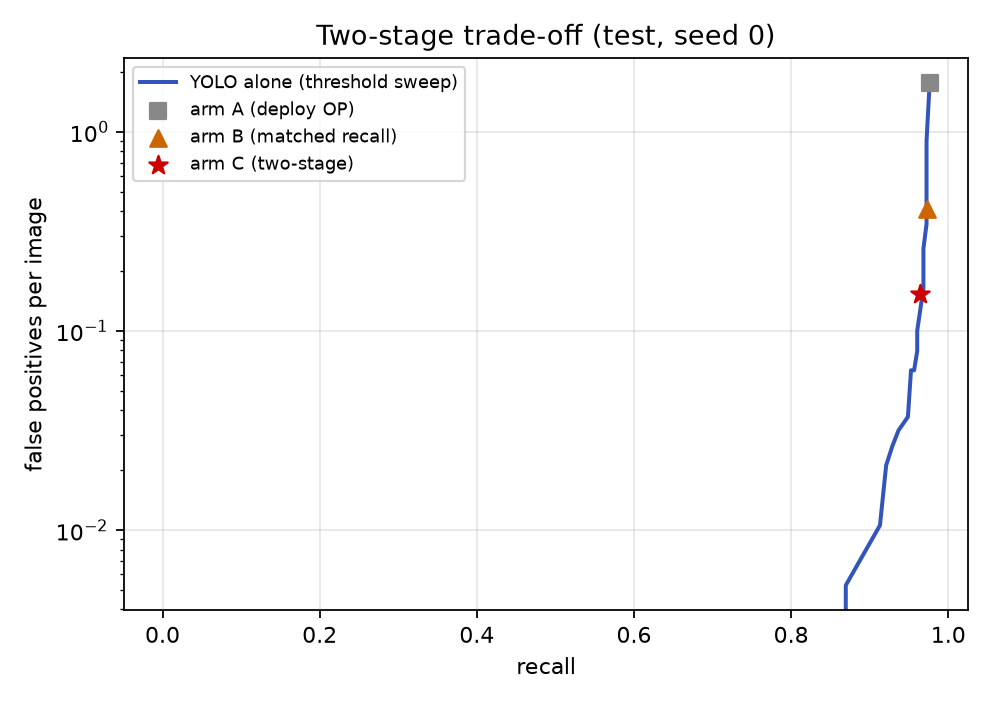
\includegraphics[width=0.78\linewidth]{figs/fp_recall_tradeoff.png}
\caption{False positives per image against recall for the single-stage and
two-stage arms (seed 0). The classifier's advantage is concentrated at high
recall; at moderate recall a tuned single-stage threshold is better. Curves are
drawn from the same frozen test records used in Table~\ref{tab:twostage}.}
\label{fig:tradeoff}
\end{figure}

\subsection{Second-stage ablations}
\label{sec:ablation}

Five variants isolate the recipe (Table~\ref{tab:ablation}). Removing hard
negatives is the largest single degradation
($\Delta P = -0.056\ [-0.084, -0.028]$), which is unsurprising given that the
negatives are detector false positives rather than random background. Removing
context padding ($0.0$) costs $0.027$ precision, and doubling it ($0.4$) costs
$0.025$: the $20\%$ margin is a genuine optimum rather than a monotone knob.
Reducing crop resolution to $160$ \emph{improves} precision by $0.017$ with an
interval that touches zero $[0.000, 0.036]$, a difference we do not claim.
Doubling to $320$ costs $0.025$. All intervals are paired image bootstraps
against the baseline on the same test images.

\begin{table}[t]
\centering
\small
\caption{Stage-2 ablations at the validation-chosen recall-safe rule, detector
seed 0. $\Delta P$ is a paired image bootstrap against the baseline; an interval
spanning zero means indistinguishable.}
\label{tab:ablation}
\begin{tabular}{lccccccc}
\toprule
variant & pad & crop & hard neg. & $\tau$ & $P$ & FP/img & $\Delta P$ [95\% CI] \\
\midrule
baseline & 0.2 & 224 & yes & 0.27 & 0.894 & 0.153 & reference \\
crop 160 & 0.2 & 160 & yes & 0.43 & 0.911 & 0.127 & $+0.017\ [0.000, 0.036]$ \\
crop 320 & 0.2 & 320 & yes & 0.08 & 0.868 & 0.196 & $-0.025\ [-0.049, -0.006]$ \\
no hard neg. & 0.2 & 224 & no & 0.35 & 0.837 & 0.254 & $-0.056\ [-0.084, -0.028]$ \\
pad 0.0 & 0.0 & 224 & yes & 0.16 & 0.866 & 0.201 & $-0.027\ [-0.043, -0.011]$ \\
pad 0.4 & 0.4 & 224 & yes & 0.25 & 0.868 & 0.196 & $-0.025\ [-0.042, -0.011]$ \\
\bottomrule
\end{tabular}
\end{table}

\subsection{Grad-CAM: evidence, not correctness}
\label{sec:gradcam}

We use attribution as a falsification tool and report what it shows, including
where it is uninformative. On $244$ true-positive detections, the median share of
CAM energy inside the ground-truth box is $0.939$ (mean $0.690$, first quartile
$0.0002$, third quartile $0.996$). Median enrichment over the box's area share is
$58.2\times$; the peak falls inside the box for $73.0\%$ of detections. The
bimodality is important: the distribution is not centred on a high value, it is
split between detections whose evidence is almost entirely on the object and
detections whose evidence is almost entirely elsewhere. The second group is
where the detector is right for the wrong reason.

Deletion tests confirm the direction. Masking the ground-truth box lowers the
detection score by $0.739$ on average ($n=182$); masking a matched background
region lowers it by $0.0015$. The detector's score depends on the object region,
as it should.

The head-to-head comparison is the cautionary result. On images where both the
detector and the image-level classifier are correct, detector enrichment has
median $86.0\times$ and the MobileNetV3 baseline has median $1.82\times$; the
paired difference is $+147.0\ [125.4, 170.0]$ in favour of the detector. On
detector crops, the stage-2 classifier reaches only $2.13\times$. The classifier
that achieves $97.4\%$ image-level accuracy is not looking at the object in any
localised sense; it is exploiting context. That does not make its decisions wrong
on this test set, but it explains why fine-tuning it adds so little precision and
why its gains vanish when the baseline threshold is already good.

\begin{figure}[t]
\centering
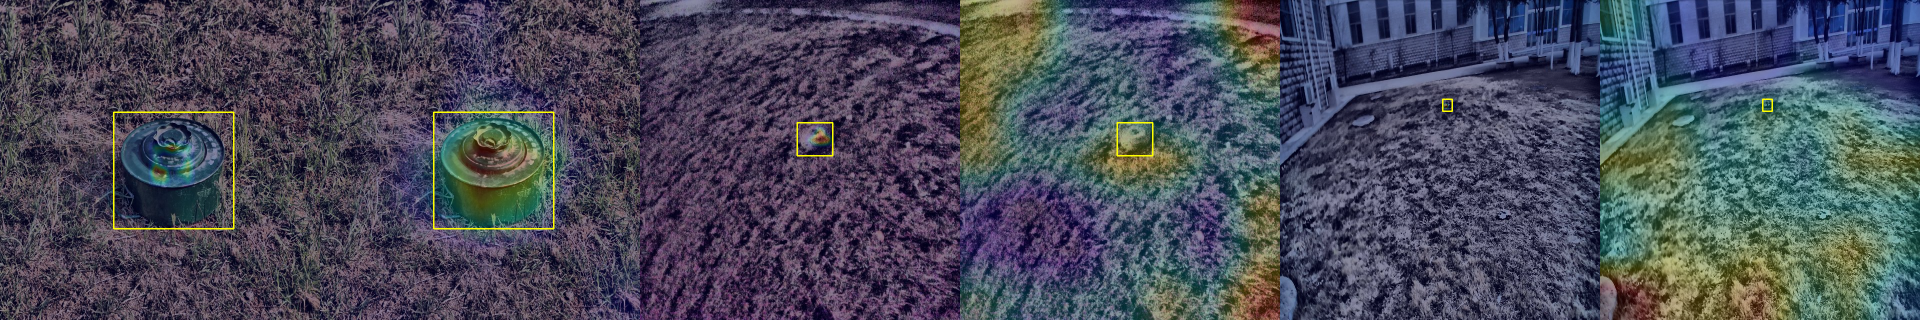
\includegraphics[width=0.95\linewidth]{figs/gradcam_example_grid.png}
\caption{Grad-CAM on detector crops (top) and image-level classifier (bottom).
The detector's evidence is object-localised; the classifier's is diffuse. This is
a statement about where each model looks, not about whether either prediction is
correct.}
\label{fig:gradcam}
\end{figure}

A paste-and-remove test probes the same question behaviourally. Pasting a mine
crop into a background yields detection at $0.650$ under the deploy confidence
and $0.630$ at the matched-recall confidence, against $0.976$ recall on original
images; inpainting a mine out of an image makes it disappear in $100$ of $100$
composites. The asymmetry is expected: synthetic pastes carry feathered edges and
scale mismatch, so the detector is being asked to fire on an object that looks
slightly wrong. We report the numbers as an upper bound on the paste setup's
realism, not as an estimate of the detector's sensitivity to context. The
zero-energy cases are more useful: exactly two test images had zero CAM energy in
the box, and both were the objectively wrong labels found in manual review. That
independent confirmation is the strongest evidence in this section that the
attribution pipeline is measuring something real.

Finally, the failure catalogue (Table~\ref{tab:failures}) is the qualitative
counterpart. Of $29$ reviewed false positives, $22$ are terrain texture; of $9$
false negatives, $5$ are camouflaged or low-contrast objects and $2$ are small.
The failure mass is where the deployment risk is, and it is not visible in any
aggregate score.

\begin{table}[t]
\centering
\small
\caption{Hand-reviewed failure categories at the arm-C deployment threshold
(seed 0). False positives are capped at $50$; $29$ were present.}
\label{tab:failures}
\begin{tabular}{lrr}
\toprule
category & FN & FP \\
\midrule
camouflaged or low contrast & 5 & 0 \\
small object & 2 & 0 \\
label error & 2 & 0 \\
terrain texture & 0 & 22 \\
low-light ground & 0 & 2 \\
fence / structure edge & 0 & 2 \\
structure wall & 0 & 1 \\
sensor noise & 0 & 1 \\
tree trunk & 0 & 1 \\
\midrule
total & 9 & 29 \\
\bottomrule
\end{tabular}
\end{table}

\begin{figure}[t]
\centering
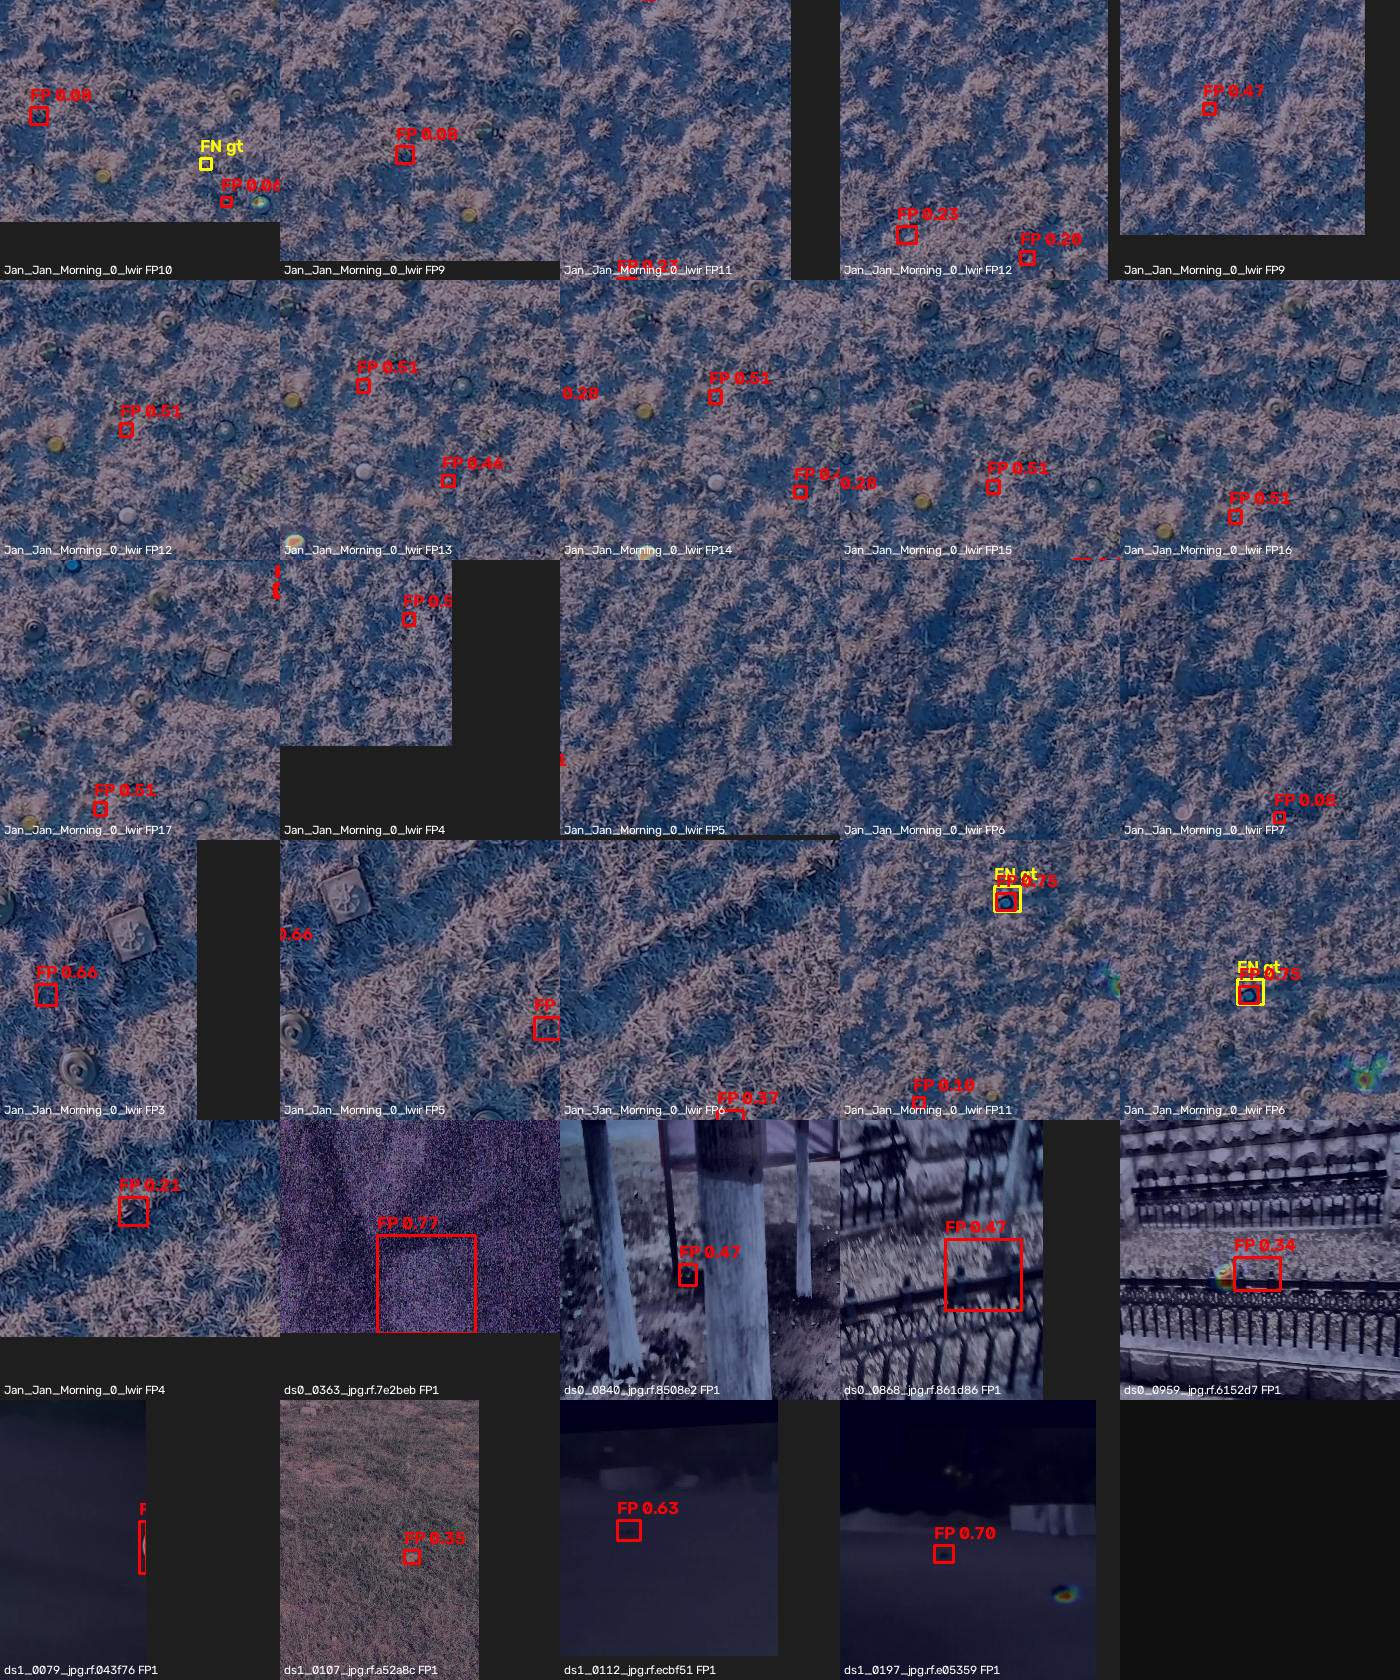
\includegraphics[width=0.62\linewidth]{figs/failure_gallery_fp.png}
\caption{Representative false positives. Terrain texture dominates; the
distinction between a mine-like disc and a rock or a patch of ground is the
failure mode that matters operationally.}
\label{fig:failures}
\end{figure}
